\documentclass[acmsmall,screen,review,anonymous,nonacm]{acmart}

\usepackage{paper}

\begin{document}

\title{Variability-Aware Analysis of Kbuild Makefiles}

\author{Anonymous Author(s)}
\affiliation{\institution{Anonymous Institution} \country{}}
\renewcommand{\shortauthors}{Anonymous Author(s)}

\begin{abstract}
  The Linux kernel is one of the most configurable software systems in computing, and its Kbuild Makefiles determine which source files are compiled and linked based on thousands of configuration options.
  To understand why a source file is omitted from a build, or which configuration options enable it, a developer requires its build condition: a propositional formula over configuration options specifying when the file is compiled.
  Evaluating Make on a single configuration answers this question for one configuration at a time, while exhaustively enumerating all configurations is intractable.
  Conventional symbolic execution forks a new execution state at every conditional branch and multi-valued option, causing exponential path explosion.
  This paper presents \tool{}, a variability-aware symbolic execution approach for Kbuild Makefiles that maintains a single consolidated symbolic state throughout Makefile evaluation.
  \tool{} maps each Make variable to a set of words, where each word carries a path condition over configuration options in the style of a value summary.
  Append statements add words with their path conditions incrementally, overwrites perform conditional updates that conjoin the negated path condition to pre-existing words, and conditional branches merge states at join points, keeping the symbolic state proportional to the number of distinct words in each variable.
  We represent the resulting build conditions as quantifier-free first-order formulae in an SMT solver to verify reachability and synthesize valid configurations.
  We evaluate \tool{} on four open-source Kbuild systems, including Linux 7.2.8 and BusyBox 1.38.0.
  On 36 concrete Linux builds across four architectures, \tool{} achieves 1.000 precision and 0.953 to 0.990 recall (compared with 0.857 to 0.913 and 0.918 to 0.962 for Kmax), while whole-tree analysis of one architecture completes in 53 to 55\,s, 5.3 to 5.5 times faster than Kmax.
\end{abstract}

\begin{CCSXML}
<ccs2012>
<concept>
<concept_id>10011007.10011074.10011099</concept_id>
<concept_desc>Software and its engineering~Software verification and validation</concept_desc>
<concept_significance>500</concept_significance>
</concept>
</ccs2012>
\end{CCSXML}
\ccsdesc[500]{Software and its engineering~Software verification and validation}
\keywords{Kbuild, Makefile, symbolic execution, variability, Kconfig}

\maketitle

\section{Introduction}
  \label{sec:intro}
  The build system determines which source files reach the compiler.
  In large-scale configurable software systems such as the Linux kernel, the build process is controlled by configuration options specified by the developer~\cite{berger2013variability,dietrich2012variability}.
  The Linux kernel provides over 14,000 configuration options that configure device drivers, file systems, network protocols, and hardware architectures.
  Building the kernel involves two distinct subsystems~\cite{nguyen2020kbuild,gazzillo2017kmax}: the Kconfig configuration system, which defines configuration options and their logical dependencies, and the Kbuild build system, which uses GNU Make to compile source files into object files and link them into kernel images and modules.
  Developers select features using an interactive configurator, which writes the chosen settings to a configuration file named \texttt{.config}.

  During kernel development and continuous integration, developers frequently need to understand how configuration options affect the build.
  When modifying a driver or writing a bug fix, a developer may run a build that compiles successfully yet omits the modified source file, because the active configuration does not select that file.
  A concrete build log and \texttt{.config} file show what was compiled for one specific configuration, but they do not distinguish why a target file was omitted, nor which configuration settings would compile it~\cite{nguyen2020kbuild}.
  Previous empirical studies document that configuration dependencies can obscure whether an option actually affects the compiled artifacts~\cite{passos2013coevolution,nadi2014mining}.
  To resolve build omissions, developers need each file's \emph{build condition}: a logical formula over configuration options specifying the exact configurations under which the file is compiled.

  Extracting build conditions from Kbuild Makefiles presents significant challenges.
  First, Kbuild Makefiles support runtime variable name construction~\cite{gazzillo2017kmax}: an assignment such as
  \texttt{obj-\$(\allowbreak CONFIG\_\allowbreak EXT4\_\allowbreak FS) += ext4.o}
  dynamically expands the configuration option to form the target variable name (\texttt{obj-y} for built-in, \texttt{obj-m} for modular, or \texttt{obj-} when disabled).
  Second, assignments may conditionally overwrite variables, so an assignment later in a Makefile can eliminate an object added earlier.
  Third, Kbuild organizes builds hierarchically by descending into subdirectories listed in target variables, so a file's build condition depends on the reachability of its enclosing directory routes.
  Fourth, multi-file targets form composite objects whose component files are declared in auxiliary variables.
  Consequently, a simple lexical scan of \texttt{CONFIG\_} names in a Makefile cannot determine whether or when an object file is built.

  Symbolic execution provides a principled technique for analyzing programs by treating inputs as symbolic variables and accumulating path conditions along execution paths~\cite{king1976symbolic}.
  Applied to build systems, configuration options serve as symbolic inputs.
  However, conventional symbolic execution forks a new execution state at each conditional branch and multi-valued option expansion~\cite{nguyen2020kbuild}.
  Because Kbuild Makefiles contain dozens of independent conditional statements, path-forking symbolic execution suffers from exponential path explosion, creating millions of paths and exceeding memory limits on real-world Makefiles.
  The pioneering static analysis tool Kmax~\cite{gazzillo2017kmax} made whole-repository Kbuild analysis feasible by tracking reaching configurations as Binary Decision Diagrams (BDDs) over complete string values.
  However, string-based representations combine alternatives via cross products during variable concatenation, which can introduce performance overhead on large Makefiles.

  In this paper, we present \tool{}, a variability-aware symbolic execution approach for Kbuild Makefiles that maintains a single consolidated symbolic state throughout Makefile evaluation.
  \tool{} is based on the insight that Kbuild target variables operate as sets of independent words.
  By mapping each Make variable to a set of words and attaching a path condition to each individual word, \tool{} represents variable contents as Boolean value summaries in the sense of MultiSE~\cite{sen2015multise}.
  Independent appends incrementally add words with their respective path conditions, while overwrite assignments perform conditional updates that narrow the path conditions of pre-existing words.
  At conditional join points, \tool{} applies static state merging~\cite{kuznetsov2012efficient,avgerinos2014enhancing} to combine branch states back into a single environment, employing an identity simplification that prevents formula growth for unmodified words.
  By offloading satisfiability checks, directory route reachability, and configuration synthesis to a satisfiability modulo theories (SMT) solver (Z3~\cite{demoura2008z3}), \tool{} extracts build conditions across entire source trees in seconds.

  This paper makes the following contributions:
  \begin{itemize}[leftmargin=1.5em]
    \item \textbf{Approach:} We formulate Kbuild Makefile evaluation as a variability-aware symbolic execution over word-level value summaries, executing statements in a single pass and merging branch states at conditional join points without auxiliary variables.
    \item \textbf{Algorithm:} We design a worklist algorithm that traverses the hierarchical Kbuild directory structure, prunes unreachable directory routes via SMT satisfiability queries, and models Kbuild build semantics including composite objects and canned rule prerequisites.
    \item \textbf{Implementation:} We implement \tool{} in Python with the Z3 SMT solver and provide developer commands to explain build omissions (\texttt{why}), synthesize minimal configurations for source patches (\texttt{config-for}), and identify uncompiled source files (\texttt{blindspots}).
    \item \textbf{Evaluation:} We evaluate \tool{} on four open-source Kbuild projects (Linux, BusyBox, Barebox, and Xen). On concrete builds of 36 Linux configurations for i386, x86-64, arm64, and arm, \tool{} matches the compiled object inventory with 1.000 precision and 0.953 to 0.990 recall, while completing the whole-tree analysis of one architecture in 53 to 55\,s, 5.3 to 5.5 times faster than Kmax.
  \end{itemize}

\section{Background}
  \label{sec:background}
  This section provides background on the Linux Kbuild build system, Kconfig configuration models, and symbolic execution with state merging.

  \subsection{Linux Kbuild and Kconfig}
    \label{sec:background:kbuild}
    The Linux kernel build infrastructure separates feature configuration from build execution~\cite{nguyen2020kbuild}.
    Configuration options are defined in Kconfig files across the source tree, which declare option types (Boolean, tristate, integer, string) and express constraints such as dependencies (\texttt{depends on}), mandatory selections (\texttt{select}), and mutual-exclusion groups (\texttt{choice}).
    A Boolean option takes the value \texttt{y} (enabled) or remains unset (disabled).
    A tristate option supports loadable kernel modules, taking \texttt{y} (compiled directly into the kernel image), \texttt{m} (compiled as a separate loadable module), or unset.
    When a developer configures the kernel using a tool such as \texttt{make menuconfig} or \texttt{make defconfig}, the selections are written to a flat text file named \texttt{.config}.

    Kbuild uses GNU Make to translate the settings in \texttt{.config} into compilation and linking commands.
    Kbuild Makefiles define compilation targets by populating reserved variables termed \emph{goal definitions}~\cite{gazzillo2017kmax}:
    \texttt{obj-y} lists object files compiled and linked into the kernel image (\texttt{vmlinux} or archive \texttt{built-in.a});
    \texttt{obj-m} lists object files compiled as loadable kernel modules;
    and \texttt{lib-y} lists archive library objects.
    Kbuild relies heavily on \emph{runtime variable name construction}, appending an option's value to the variable prefix:
    \begin{lstlisting}[style=kbuild]
    obj-$(CONFIG_EXT4_FS) += ext4.o
    \end{lstlisting}
    When \texttt{CONFIG\_EXT4\_FS} is \texttt{y}, Make expands the destination to \texttt{obj-y}; when it is \texttt{m}, it expands to \texttt{obj-m}; and when unset, it expands to \texttt{obj-}, which Kbuild ignores.

    Kbuild also manages multi-file targets through \emph{composite objects}.
    When a target object \texttt{foo.o} is composed of multiple compilation units, the Makefile defines the constituent files using variables named \texttt{foo-y} or \texttt{foo-objs}:
    \begin{lstlisting}[style=kbuild]
    obj-$(CONFIG_FOO) += foo.o
    foo-y             := file1.o file2.o
    \end{lstlisting}
    Furthermore, Kbuild organizes compilation hierarchically by \emph{descending into subdirectories}.
    When an entry in a goal definition ends with a slash, such as \texttt{obj-\$(CONFIG\_DRIVERS) += drivers/}, Kbuild recurses into \texttt{drivers/Makefile}.

  \subsection{Symbolic Execution and State Merging}
    \label{sec:background:symex}
    Symbolic execution evaluates a program by supplying symbolic variables in place of concrete input values~\cite{king1976symbolic}.
    An execution state maintains a symbolic store mapping variables to symbolic expressions, alongside a path condition: a first-order logic formula that accumulates the branch conditions satisfied along the current execution path.
    A path condition is satisfiable if there exists at least one concrete input assignment that follows that path.

    In conventional dynamic or static symbolic execution, encountering a conditional branch with symbolic test condition $\kappa$ forks the execution state into two independent paths: one exploring the then-arm under path condition $g \land \kappa$, and another exploring the else-arm under $g \land \neg\kappa$.
    When a program contains $k$ sequential, independent branches, path forking generates $2^k$ distinct execution paths, leading to path explosion.
    To mitigate path explosion, \emph{state merging} combines the symbolic states of converging paths at join points~\cite{kuznetsov2012efficient,avgerinos2014enhancing}.
    Traditional state merging introduces auxiliary variables and if-then-else expressions at join points, which can increase formula complexity for downstream constraint solvers.
    MultiSE~\cite{sen2015multise} introduced \emph{value summaries}, mapping each program variable to a set of conditional value expressions $\{(\phi_1, v_1), (\phi_2, v_2), \dots\}$ where the path conditions $\phi_i$ partition the configuration space.
    MultiSE updates value summaries incrementally at every assignment and performs conditional updates during overwrites, avoiding auxiliary variables.
    In this paper, we adapt value summaries and state merging to the domain of Kbuild Makefiles, treating target variables as sets of independent words.

\section{Motivating Example}
  \label{sec:example}
  This section walks through the symbolic execution of a Kbuild Makefile in \tool{} to illustrate how build conditions are computed and how the consolidated symbolic state remains compact.
  \autoref{lst:example} shows a Kbuild Makefile adapted from the Linux \texttt{ext4} file system.
  A developer who modifies a source file in this directory and runs a build may ask why \texttt{ext4.o} was omitted from the build, or which configuration settings would compile it.
  Running Make with a single \texttt{.config} file answers this question for one configuration at a time.
  A build condition summarizes this behavior across the configuration space as a logical constraint over configuration options that specifies when the file is included in the build.

  \begin{figure}[t]
  \begin{lstlisting}[style=kbuild]
  obj-$(CONFIG_EXT4_FS) += ext4.o
  obj-$(CONFIG_EXT4_KUNIT_TESTS) := ext4-inode-test.o
  ifeq ($(CONFIG_FS_VERITY),y)
    EXTRA := verity
  else
    EXTRA := crypto
  endif
  obj-y += $(EXTRA).o
  ext4-inode-test-y += inode-test.o
  \end{lstlisting}
  \caption{Makefile adapted from Linux \texttt{fs/ext4/Makefile}. Only line~1 is verbatim; lines~2 and~9 are adapted and lines~3--8 are constructed to add an overwrite, a conditional, and a composite object.}
  \Description{A nine-line Kbuild Makefile with an append, an overwrite, a conditional assignment, and a composite file.}
  \label{lst:example}
  \end{figure}

  Let the symbolic variables $E$, $T$, and $V$ denote the configuration options \texttt{CONFIG\_EXT4\_FS}, \texttt{CONFIG\_\allowbreak EXT4\_\allowbreak KUNIT\_\allowbreak TESTS}, and \texttt{CONFIG\_FS\_VERITY}, respectively.
  \tool{} treats configuration options as symbolic inputs and executes the Makefile over a single consolidated symbolic state.
  Each Make variable is mapped to a set of words, where each word carries a path condition over configuration options in the style of a Boolean value summary~\cite{sen2015multise} (and a variational set of words~\cite{walkingshaw2014variational}).
  Line~1 expands the left-hand side and appends \texttt{ext4.o} to \texttt{obj-y} under path condition $E = \mathtt{y}$ and to \texttt{obj-m} under path condition $E = \mathtt{m}$.
  Line~2 is a conditional overwrite whose left-hand side also depends on a configuration option: under $T = \mathtt{y}$ it overwrites \texttt{obj-y} with \texttt{ext4-inode-test.o}, and under $T = \mathtt{m}$ it overwrites \texttt{obj-m}.
  To preserve existing words on configurations where the overwrite does not take effect, \tool{} performs a conditional update~\cite{sen2015multise,gazzillo2017kmax}: it adds \texttt{ext4-inode-test.o} to \texttt{obj-y} under $T = \mathtt{y}$ and to \texttt{obj-m} under $T = \mathtt{m}$, while conjoining the negated condition with prior entries, so \texttt{ext4.o} remains in \texttt{obj-y} under $(E = \mathtt{y}) \land (T \ne \mathtt{y})$ and in \texttt{obj-m} under $(E = \mathtt{m}) \land (T \ne \mathtt{m})$.
  Lines~3--7 assign \texttt{EXTRA} in both arms of an \texttt{ifeq} conditional; at the join point, state merging combines the two arms into a single symbolic state mapping \texttt{EXTRA} to \texttt{verity} under $V = \mathtt{y}$ and to \texttt{crypto} under $V \ne \mathtt{y}$.
  Line~8 expands \texttt{\$(EXTRA)} and concatenates each alternative with \texttt{.o}, appending two words with complementary path conditions to \texttt{obj-y}.
  Finally, line~9 defines \texttt{inode-test.o} as a member of the composite object \texttt{ext4-inode-test.o}, which inherits the build condition of its parent composite.
  \autoref{tab:example} lists the resulting build conditions.
  These conditions are local to \texttt{fs/ext4/Makefile}; the full build condition of each file conjoins the directory path condition under which Kbuild descends into \texttt{fs/ext4/}.

  \begin{table}[t]
  \centering\footnotesize
  \caption{Build conditions of the files built by \autoref{lst:example}.}
  \label{tab:example}
  \begin{tabular}{lll}
  \toprule
  File & Built into the kernel (\texttt{obj-y}) & Built as a module (\texttt{obj-m}) \\
  \midrule
  \texttt{ext4.o} & $(E = \mathtt{y}) \land (T \ne \mathtt{y})$ & $(E = \mathtt{m}) \land (T \ne \mathtt{m})$ \\
  \texttt{ext4-inode-test.o} & $T = \mathtt{y}$ & $T = \mathtt{m}$ \\
  \texttt{inode-test.o} & $T = \mathtt{y}$ & $T = \mathtt{m}$ \\
  \texttt{verity.o} & $V = \mathtt{y}$ & --- \\
  \texttt{crypto.o} & $V \ne \mathtt{y}$ & --- \\
  \bottomrule
  \end{tabular}
  \end{table}

  Representing build conditions as quantifier-free first-order formulae allows \tool{} to answer developer queries directly with a satisfiability modulo theories (SMT) solver.
  Evaluated against a concrete \texttt{.config}, the formula for \texttt{ext4.o} explains why the file was excluded from the build, \eg, because $T = \mathtt{y}$ holds and overwrote \texttt{obj-y}.
  Conjoined with the feature-model constraints extracted from Kconfig, the formula enables an SMT solver to find a satisfying assignment that compiles \texttt{ext4.o} by satisfying $(E = \mathtt{y}) \land (T \ne \mathtt{y})$.
  \tool{} exposes these analyses through the \texttt{why} and \texttt{config-for} commands; \autoref{sec:eval} validates the solver-generated configurations with the kernel configurator and concrete builds.

  Prior symbolic execution of Kbuild Makefiles by Nguyen and Nguyen~\cite{nguyen2020kbuild} follows conventional path-based exploration: it forks a new execution state at every conditional or multi-valued expansion and mitigates path explosion by combining execution paths and applying a split-merge strategy~\cite{avgerinos2014enhancing,sen2015multise}.
  On \autoref{lst:example}, expanding the two tristate options and branching on the conditional spawns $3 \times 3 \times 2 = 18$ execution paths before merging, and each subsequent independent conditional can double the path count.
  \tool{} maintains a single consolidated symbolic state in which \texttt{obj-y} and \texttt{obj-m} hold six words in total, and each subsequent append adds only the new words with their path conditions.
  MultiSE~\cite{sen2015multise} introduced value summaries to share symbolic expressions across paths without auxiliary variables, and Kmax~\cite{gazzillo2017kmax} similarly localizes configuration explosion to individual statements by tracking reaching configurations over complete strings.

  In summary, representing variables as sets of words with path conditions and merging states at conditional join points yields per-file build conditions at a cost proportional to the number of distinct words, enabling constraint-based reasoning over the build system.

\section{Approach}
  \label{sec:approach}
  This section presents the design and algorithms of \tool{}.
  We first formalize the problem setting, define the central notion of a build condition, and introduce the word-level symbolic state representation (\autoref{sec:approach:state}).
  We then describe the intra-Makefile symbolic executor (\textsc{Exec}), which evaluates assignments, expands expressions, and merges branch states at conditionals in a single pass (\autoref{sec:approach:intra}).
  Next, we present the whole-tree traversal algorithm that propagates reachability conditions across directories and prunes explored routes via SMT queries (\autoref{sec:approach:dirs}).
  Finally, we detail how extracted words are resolved into physical object files and how developer build queries are answered using constraint solving (\autoref{sec:approach:objects}).

  \subsection{Problem Formulation and Symbolic State}\label{sec:approach:state}
  We begin by formalizing the configuration space and the build condition that \tool{} computes.
  A software project $M$ governed by Kbuild is parameterized by a finite set of configuration options $\mathcal{X} = \{x_1, \dots, x_k\}$.
  Each option $x_i$ takes a value from a discrete domain $\mathcal{D}(x_i)$ determined by its Kconfig type: Boolean options range over $\{\mathtt{y}, \bot\}$ (where $\bot$ denotes unset), and tristate options range over $\{\mathtt{y}, \mathtt{m}, \bot\}$, where $\mathtt{m}$ denotes a loadable kernel module.
  A concrete configuration $c$ is a total assignment $c : \mathcal{X} \to \bigcup_{i} \mathcal{D}(x_i)$ satisfying $c(x_i) \in \mathcal{D}(x_i)$.
  We denote the space of all valid configurations as $\mathcal{C}$.

  \begin{definition}[Build Condition]\label{def:build-condition}
  Let $M$ be a project source tree and $o$ be a target object file.
  The \emph{build condition} of $o$, denoted $\Phi_M(o)$, is a quantifier-free first-order logic formula over symbolic configuration options $\mathcal{X}$ such that for every concrete configuration $c \in \mathcal{C}$:
  \[
    c \models \Phi_M(o) \iff \text{Kbuild compiles and links } o \text{ under configuration } c.
  \]
  \end{definition}

  Intuitively, $\Phi_M(o)$ captures the complete set of configuration constraints required to build $o$: from top-level directory reachability and nested Makefile traversal to conditional goal definitions and composite object inclusion.
  When an object file is never compiled under any configuration, its build condition simplifies to false ($\Phi_M(o) = \bot$).

  To compute build conditions across all configurations simultaneously without path forking, \tool{} requires an abstract state representation tailored to GNU Make semantics.
  In Kbuild Makefiles, variables store whitespace-separated sequences of words (file paths, directory names, and compiler flags).
  Crucially, target variables operate as sets of independent words.
  \tool{} therefore represents the symbolic state $\sigma$ as an abstract symbol table mapping each variable name $n$ to a set of words, where each word $w$ is associated with a path condition $\phi_w$:
  $$\sigma[n] = \{ w \mapsto \phi_w \}$$
  Here, the path condition $\phi_w$ is a quantifier-free Boolean formula over symbolic configuration options $\mathcal{X}$.
  An entry $w \mapsto \phi$ indicates that word $w$ is present in variable $n$ under all configurations satisfying $\phi$.
  This formulation corresponds to a Boolean value summary~\cite{sen2015multise} over word membership (and a variational set of words~\cite{walkingshaw2014variational}).
  Unlike value summaries over scalar variables in imperative programs whose values are mutually exclusive, Make variables can hold multiple words simultaneously under a single configuration (\eg, \texttt{obj-y := a.o b.o}), so the path conditions of distinct words in $\sigma[n]$ may overlap.

  We write $\sigma[n](w) = \bot$ when word $w$ is absent from $\sigma[n]$.
  The join operator $\sqcup$ computes the union of two word sets, coalescing duplicate words by taking the disjunction of their path conditions:
  $$(w \mapsto \phi) \sqcup (w \mapsto \phi') = (w \mapsto \phi \lor \phi')$$
  and removing any entry whose path condition simplifies to false ($\bot$)~\cite{sen2015multise}.
  Restricting a symbolic state $\sigma$ to a condition $\delta$ conjoins $\delta$ with the path condition of every word in every variable: $\sigma|_\delta[n] = \{w \mapsto \phi \land \delta : (w \mapsto \phi) \in \sigma[n]\}$.

  \subsection{Single-Pass Intra-Makefile Execution}\label{sec:approach:intra}
  \label{sec:approach:assign}\label{sec:approach:expand}\label{sec:approach:merge}
  This subsection presents the intra-Makefile symbolic executor (\textsc{Exec}), which evaluates the statements of an individual Makefile in a single pass under an ambient path condition without forking execution paths.

  \autoref{alg:exec} (\textsc{Exec}) executes statements sequentially under an ambient path condition $g$, which represents the conjunction of enclosing conditional branches (the reaching configuration~\cite{gazzillo2017kmax}).

  \begin{algorithm}[t]
  \caption{\textsc{Exec}: symbolic execution of one statement}\label{alg:exec}
  \KwIn{statement $s$, state $\sigma$, ambient path condition $g$}
  \KwOut{updated state $\sigma$}
  \uIf{$s$ is an assignment $x\ \mathit{op}\ e$}{
    $V \gets$ the words $w \mapsto \phi_w$ of $e$ (or $e \mapsto \top$ if recursively expanded)\;\label{line:rhs}
    \ForEach{name $n$ with path condition $\psi_n$ in the expansion of $x$}{\label{line:lhs}
      $\psi \gets g \land \psi_n$\;
      \uIf{$\mathit{op}$ is an overwrite or $\sigma[n]$ is undefined}{
        $\sigma[n] \gets \{w \mapsto \psi \land \phi_w\} \sqcup \{w \mapsto \phi \land \neg\psi : (w \mapsto \phi) \in \sigma[n]\}$\;\label{line:overwrite}
      }
      \Else{
        $\sigma[n] \gets \sigma[n] \sqcup \{w \mapsto \psi \land \phi_w\}$\;\label{line:append}
      }
    }
  }
  \ElseIf{$s$ is a conditional with test $t$, then-arm $T$, else-arm $F$}{
    $\kappa \gets$ condition under which $t$ holds; $\sigma_t, \sigma_e \gets$ copies of $\sigma$\;\label{line:copy}
    $\textsc{Exec}(T,\sigma_t,g\land\kappa)$; $\textsc{Exec}(F,\sigma_e,g\land\neg\kappa)$\;
    \ForEach{name $n$ assigned in $T$ or $F$ and word $w$}{\label{line:mergeloop}
      \uIf{$\sigma_t[n](w) = \sigma_e[n](w) = \phi$}{$\sigma[n](w) \gets g \land \phi$\;\label{line:same}}
      \Else{$\sigma[n](w) \gets (g \land \kappa \land \sigma_t[n](w)) \lor (g \land \neg\kappa \land \sigma_e[n](w))$\;\label{line:merge}}
    }
  }
  \Return $\sigma$\;
  \end{algorithm}

  \emph{Dynamic LHS names and assignments.}
  GNU Make allows variable names on the left-hand side of an assignment to be computed dynamically, as in \texttt{obj-\$(CONFIG\_EXT4\_FS)}.
  \autoref{line:lhs} expands the left-hand expression $x$ into concrete variable names $n$ paired with their path conditions $\psi_n$: \texttt{obj-y} under $E = \mathtt{y}$, \texttt{obj-m} under $E = \mathtt{m}$, and \texttt{obj-} when unset.
  A single assignment statement can thus update multiple target variables under different effective path conditions $\psi = g \land \psi_n$.
  For append assignments (\texttt{+=}), \autoref{line:append} adds the right-hand words $V$ directly into $\sigma[n]$, conjoining each word's path condition $\phi_w$ with the assignment condition $\psi$: $\sigma[n] \gets \sigma[n] \sqcup \{w \mapsto \psi \land \phi_w\}$.
  For overwrite assignments (\texttt{:=} and \texttt{=}), the overwrite applies only on configurations satisfying $\psi$; on configurations satisfying $\neg\psi$, the variable retains its pre-existing words.
  \autoref{line:overwrite} therefore performs a \emph{conditional update}~\cite{sen2015multise,gazzillo2017kmax}:
  $$\sigma[n] \gets \{w \mapsto \psi \land \phi_w\} \sqcup \{w \mapsto \phi \land \neg\psi : (w \mapsto \phi) \in \sigma[n]\}$$
  In \autoref{lst:example}, line~2 overwrites \texttt{obj-y} under $\psi = (T = \mathtt{y})$, narrowing the path condition of \texttt{ext4.o} from $E = \mathtt{y}$ to $(E = \mathtt{y}) \land \neg(T = \mathtt{y})$.
  Conjoining $\neg\psi$ ensures that \texttt{ext4.o} is excluded under $(E = \mathtt{y}) \land (T = \mathtt{y})$, matching concrete Make evaluation where the second assignment discards the earlier value.

  \emph{Variable flavors.}
  \tool{} distinguishes simply-expanded variables (\texttt{:=}) from recursively-expanded variables (\texttt{=}), following SYMake~\cite{tamrawi2012symmake} and Kmax~\cite{gazzillo2017kmax}.
  A simply-expanded variable evaluates its right-hand side immediately at assignment time.
  A recursively-expanded variable stores its right-hand expression verbatim and defers evaluation until the variable is referenced; \tool{} stores an unexpanded expression when a recursive definition contains variable references (\autoref{line:rhs}) and expands deferred references in goal definitions after executing the Makefile.
  Linux's \texttt{drivers/xen/Makefile} illustrates why deferred expansion is needed: it appends \texttt{\$(xen-pad-y)} to \texttt{dom0-y} one line before defining \texttt{xen-pad-y}, so only expansion at reference time resolves \texttt{xen-acpi-pad.o}.
  \autoref{tab:scope} summarizes the Make constructs that \tool{} interprets and their analysis boundaries.

  \begin{table}[t]
  \centering\footnotesize
  \caption{Make constructs and their interpretation.}
  \label{tab:scope}
  \begin{tabular}{p{26mm}p{45mm}p{50mm}}
  \toprule
  Construct & Interpretation & Boundary \\
  \midrule
  \texttt{+=}, \texttt{=}, \texttt{:=} & Words with path conditions; the flavor decides when the right-hand side is expanded & Word order and duplicates are not kept. \\
  \texttt{ifeq}, \texttt{ifneq}, \texttt{ifdef}, \texttt{ifndef} & Both arms are executed and the states are merged & --- \\
  Variable references & Words with path conditions, or the empty word when none is present & --- \\
  \texttt{include} & The directive is replaced by the statements of the file & A path that cannot be resolved statically contributes nothing. \\
  Rules and sub-makes & Prerequisites are followed from selected objects & Other recipes are not executed. \\
  \texttt{\$(shell ...)} & A concrete subprocess & The host environment can change the result. \\
  \bottomrule
  \end{tabular}
  \end{table}

  \emph{Expansion of names and words.}
  In GNU Make, the right-hand side of an assignment is whitespace-delimited into independent words.
  Adjacent subexpressions in a token (\eg, \texttt{\$(EXTRA).o} in line~8 of \autoref{lst:example}) are concatenated with a lifted cross product~\cite{gazzillo2017kmax} that pairs each string combination with the conjunction of their path conditions, yielding \texttt{verity.o} under $V = \mathtt{y}$ and \texttt{crypto.o} under $V \ne \mathtt{y}$.
  Treating a whitespace-separated list such as \texttt{\$(a-y) \$(b-y) \$(c-y)} as a set of independent words avoids taking the cross product across the three variables, preserving each word's path condition directly.
  When a variable reference may be undefined along some paths, \tool{} includes the empty string under the negation of the variable's definedness condition, which is essential when the reference appears inside a word or list.
  For instance, Linux's \texttt{dvb-core} Makefile defines \texttt{dvb-net-\$(CONFIG\_DVB\_NET) := dvb\_net.o} and includes \texttt{\$(dvb-net-y)} in \texttt{dvb-core-objs}; retaining the empty alternative ensures that the remaining members of \texttt{dvb-core-objs} do not spuriously acquire a dependency on \texttt{CONFIG\_DVB\_NET}.
  Built-in text functions and substitution references such as \texttt{ixgbe-\$(CONFIG\_FCOE:m=y)} are lifted similarly by applying the string transformation to each word while preserving its path condition.
  Finally, \tool{} inlines \texttt{include} directives whose target paths resolve statically and slices away variable assignments that cannot flow into goal definitions or build rules.

  \emph{State merging at conditionals.}
  For an \texttt{ifeq} or \texttt{ifneq} directive, \tool{} expands both operands and computes the branch condition $\kappa$ as the disjunction of conjunctions over matching (or non-matching) words; for \texttt{ifdef} and \texttt{ifndef}, $\kappa$ is the disjunction of path conditions under which the variable has a non-empty definition~\cite{gazzillo2017kmax}.
  Chains of \texttt{else ifeq} directives are desugared into nested conditionals in the else-arm.

  To evaluate a conditional without forking paths, \tool{} clones the incoming state $\sigma$ into $\sigma_t$ and $\sigma_e$ (\autoref{line:copy}), executes the then-arm under $g \land \kappa$ and the else-arm under $g \land \neg\kappa$, and merges the resulting branch states at the confluence point (\autoref{line:merge}), following static state merging~\cite{kuznetsov2012efficient,avgerinos2014enhancing}.
  Only variables modified in either branch are iterated over during the merge (\autoref{line:mergeloop}).
  In \autoref{lst:example}, the then-arm assigns \texttt{verity} under $V = \mathtt{y}$ to \texttt{EXTRA} and the else-arm assigns \texttt{crypto} under $V \ne \mathtt{y}$, so the merged state maps \texttt{EXTRA} to both words and execution proceeds with a single symbolic state.

  Whenever a word $w$ of a modified variable $n$ carries the identical path condition $\phi$ in both branches ($\sigma_t[n](w) = \sigma_e[n](w) = \phi$), \tool{} simplifies its merged path condition directly to $g \land \phi$ (\autoref{line:same}).
  Factoring $(g \land \kappa \lor g \land \neg\kappa) \land \phi \equiv g \land \phi$ avoids wrapping previously added words in case splits.
  This identity merge is critical for scalability: in a Makefile with $k$ sequential conditionals that each append an object to \texttt{obj-y}, unmodified entries do not accumulate redundant disjunctive branch conditions.

  \begin{proposition}\label{prop:merge}
  Let $\sigma'$ be the symbolic state that \autoref{alg:exec} produces after a conditional statement with branch condition $\kappa$ under ambient path condition $g$.
  For every configuration $c$ satisfying $g \land \kappa$, $\sigma'$ evaluates to the same word set as the then-arm state $\sigma_t$, and for every configuration $c$ satisfying $g \land \neg\kappa$, $\sigma'$ evaluates to the same word set as the else-arm state $\sigma_e$.
  \end{proposition}

  \noindent
  \autoref{prop:merge} holds for the core calculus of assignments and conditionals in \autoref{alg:exec}, where word order and multiplicity are abstracted.
  The proof follows from \autoref{line:merge} by distributing evaluation under $c$ across the disjunction $(g \land \kappa \land \sigma_t[n](w)) \lor (g \land \neg\kappa \land \sigma_e[n](w))$; when $\sigma_t[n](w) = \sigma_e[n](w) = \phi$, factoring out $\phi$ yields $(g \land \kappa \lor g \land \neg\kappa) \land \phi \equiv g \land \phi$ (\autoref{line:same}).
  \tl{full proof in the supplementary material}

  \subsection{Whole-Tree Traversal and Directory Descent}\label{sec:approach:dirs}
  This subsection presents the whole-tree traversal algorithm that propagates reachability conditions across the directory hierarchy of a source tree.

  In Kbuild, listing a directory in a goal definition, \eg, \texttt{obj-\$(CONFIG\_X) += sub/}, instructs Make to descend into \texttt{sub/} and evaluate \texttt{sub/Makefile}, paralleling the directory structure of the source tree~\cite{gazzillo2017kmax}.
  \tool{} propagates the path condition of the directory entry as the incoming path condition $\gamma$ for the child Makefile, so every object and subdirectory in the child inherits its parent's reachability constraint.

  \begin{algorithm}[t]
  \caption{Build conditions of the objects of a source tree}\label{alg:extract}
  \KwIn{entry Makefiles $E$ with their path conditions, goal-definition prefixes $\Gamma$}
  \KwOut{map $\Phi$ from objects to build conditions}
  $R[m] \gets \bot$ for each Makefile $m$; $Q \gets E$; $\Phi[o] \gets \bot$ for each object $o$\;
  \While{$Q$ is nonempty}{\label{line:loop}
    remove $(m,\gamma)$ from $Q$\;
    $\delta \gets \gamma \land \neg R[m]$\;\label{line:delta}
    \lIf{$\delta$ is unsatisfiable}{\textbf{continue}}\label{line:skip}
    $S \gets$ state of $m$ after \textsc{Exec}, restricted to $\delta$\;\label{line:exec}
    $R[m] \gets R[m] \lor \gamma$\;\label{line:covered}
    \ForEach{subdirectory $d$ with path condition $\eta$ in $S$}{
      add (Makefile of $d$, $\eta$) to $Q$\;\label{line:descend}
    }
    \ForEach{object $(o,\phi)$ selected by $S$ through $\Gamma$}{
      $\Phi[o] \gets \Phi[o] \lor \phi$\;\label{line:object}
    }
  }
  \Return $\textsc{Close}(\Phi)$\tcp*{objects that rules need}\label{line:close}
  \end{algorithm}

  A subdirectory Makefile can be reached along multiple directory routes.
  For instance, if a parent Makefile selects \texttt{a/} under path condition $A$ and \texttt{b/} under path condition $B$, and both \texttt{a/Makefile} and \texttt{b/Makefile} select \texttt{shared/}, then an object \texttt{x.o} unconditionally listed in \texttt{shared/Makefile} has the build condition $A \lor B$.
  Marking \texttt{shared/Makefile} as visited after traversing \texttt{a/} would miss the reachability path through \texttt{b/}.

  To handle multiple routes and cycles, \autoref{alg:extract} maintains a table $R[m]$ for each Makefile $m$ recording the cumulative path condition of configurations already explored (\autoref{line:covered}).
  When $(m, \gamma)$ is dequeued from worklist $Q$, the algorithm computes the residual path condition $\delta = \gamma \land \neg R[m]$ of unexplored configurations (\autoref{line:delta}).
  If $\delta$ is unsatisfiable (checked with Z3), no new configurations reach $m$ and the visit is pruned (\autoref{line:skip}); otherwise, \tool{} evaluates $m$ under $\delta$ via \textsc{Exec} and disjoins $\gamma$ into $R[m]$.
  Consequently, cyclic directory references terminate as soon as their residual condition becomes unsatisfiable, and because both the set of Makefiles and the configuration space are finite, $R[m]$ can be weakened only finitely many times before the worklist empties.
  Because top-level project Makefiles primarily contain imperative build recipes and environment setup, \tool{} starts traversal from the entry Makefiles specified in the project settings (\autoref{sec:impl}).

  \subsection{Object Resolution and Build Condition Reasoning}\label{sec:approach:objects}
  \label{sec:approach:use}\label{sec:approach:meaning}
  This subsection details how \tool{} translates extracted words into physical compiled objects and formulates developer queries as SMT problems over build conditions.

  \emph{From words to physical objects.}
  While goal definitions specify which compilation units and composites are selected, Kbuild's linking rules determine which physical \texttt{.o} files are emitted on disk.
  \tool{} inspects variables whose names match the goal-definition prefixes (\eg, \texttt{obj-}, \texttt{lib-}) configured for the project, suffixed by \texttt{y}, \texttt{m}, or the empty suffix.
  When a goal definition selects a composite object $t$\texttt{.o}, Kbuild resolves its component member objects from the variables $t$\texttt{-y} and $t$\texttt{-objs}, and additionally from $t$\texttt{-m} when $t$ is built as a module.
  Each member object is compiled under the conjunction of its own membership path condition and the build condition of the parent composite $t$, as illustrated by \texttt{inode-test.o} in \autoref{tab:example}.
  Composite expansion accounts for a large fraction of the kernel build: in Linux, 16,336 of the 32,829 extracted objects are members of composite objects.
  Beyond basic goal definitions and composites, \tool{} models three Kbuild semantics that govern object emission:
  \begin{itemize}[leftmargin=1.5em]
    \item \emph{Built-in composite objects:} When a composite object is selected via \texttt{obj-y} to be linked directly into the kernel image, Kbuild compiles its member objects and links them into the parent archive without emitting an intermediate $t$\texttt{.o} file; accordingly, \tool{} emits the composite object $t$\texttt{.o} itself only under the path condition for which it is selected as a module via \texttt{obj-m}.
    \item \emph{Routes into directories:} Kbuild compiles the built-in (\texttt{obj-y}) objects of a subdirectory only when the subdirectory is reached through a chain of \texttt{obj-y} directory entries (tracked by Kbuild's internal \texttt{need-builtin} flag); if a parent Makefile enters the subdirectory solely via \texttt{obj-m}, only module targets in that subdirectory are built. \tool{} therefore tracks separate built-in and module path conditions for each Makefile.
    \item \emph{Rule prerequisites:} Certain object files, such as linker scripts, generated offsets, and boot stubs, are never listed in goal definitions and are compiled solely because an explicit Makefile rule or sub-make command depends on them. During symbolic execution, \tool{} records explicit rules (mapping expanded targets to prerequisites under their ambient path conditions~\cite{gazzillo2017kmax,tamrawi2012symmake}) as well as sub-make invocations that specify a target directory and goal; after worklist traversal, \textsc{Close} (\autoref{line:close}) computes the transitive closure of prerequisites starting from all selected objects and top-level link targets such as \texttt{vmlinux.o}.
  \end{itemize}

  \emph{Domain encoding and static boundaries.}
  Each symbolic configuration option ranges over the values declared by its Kconfig type: a Boolean option ranges over $\{\mathtt{y}, \bot\}$, while a tristate option ranges over $\{\mathtt{y}, \mathtt{m}, \bot\}$ and conjoins the global module-support constraint \texttt{CONFIG\_MODULES=y} with every \texttt{=m} predicate.
  An extracted build condition $\Phi_M(o)$ is a static approximation of Kbuild's concrete behavior: \tool{} models the Kbuild subset of GNU Make shown in \autoref{tab:scope} and initiates traversal from the declared entry Makefiles, leaving arbitrary shell recipes and top-level orchestration rules outside the analysis.
  Moreover, $\Phi_M(o)$ captures the constraints encoded in Kbuild Makefiles alone; Kconfig inter-option dependencies (\texttt{depends on}, \texttt{select}, and \texttt{choice} blocks) are conjoined separately during solver queries.
  Consequently, any satisfying assignment produced by the SMT solver is treated as a candidate configuration that must be validated by running the Kconfig configurator and executing a concrete build, as evaluated in \autoref{sec:eval}.

  \emph{Reasoning with build conditions.}
  Because each build condition $\Phi_M(o)$ is a quantifier-free first-order formula over symbolic configuration options, reasoning about when an object is built reduces to evaluating or solving $\Phi_M(o)$ with an SMT solver~\cite{nguyen2020kbuild}:
  \begin{itemize}[leftmargin=1.5em]
    \item \emph{Explaining build omissions} (\texttt{why}): The \texttt{why} command takes an object file and a concrete \texttt{.config}, evaluates $\Phi_M(o)$ under that configuration's option assignments, and reports both the resulting build status and a condition chain highlighting which option clauses in $\Phi_M(o)$ are violated.
    \item \emph{Configuration synthesis} (\texttt{config-for}): The \texttt{config-for} command takes a commit or patch, maps the modified C and assembly source files to their corresponding target objects, conjoins their build conditions with the Kconfig feature-model constraints for the relevant options, and queries the SMT solver for a satisfying configuration that minimizes the number of option changes relative to a baseline \texttt{.config}. If two modified files require mutually exclusive configuration settings, the conjunction is unsatisfiable and \tool{} partitions the targets into compatible groups so each can be tested in a separate build.
    \item \emph{Uncompiled source identification} (\texttt{blindspots}): Maintainers can query for source files whose corresponding target object has an unsatisfiable build condition ($\Phi_M(o) = \bot$). These indicate dead code or broken build rules within the current architecture.
  \end{itemize}

\section{Implementation}\label{sec:impl}

This section describes the implementation of \tool{}, its project configuration format, and its command-line analyses.
\tool{} is implemented in Python.
Following Kmax~\cite{gazzillo2017kmax} and Nguyen and Nguyen~\cite{nguyen2020kbuild}, it parses Makefiles into abstract syntax trees (ASTs) using \texttt{pymake3}, our Python~3 port of the Mozilla \texttt{pymake} parser, and represents path conditions and build conditions as quantifier-free formulae in the Z3 SMT solver~\cite{demoura2008z3}.
Each configuration option is encoded as a finite enumeration sort in Z3 over two values ($\{\texttt{y}, \text{unset}\}$ for the Boolean domain) or three values ($\{\texttt{y}, \texttt{m}, \text{unset}\}$ for projects that enable the tristate domain).
Path conditions are constructed from equality predicates over these option sorts using logical conjunction, disjunction, and negation, and \tool{} simplifies each formula eagerly after every Boolean operation~\cite{sen2015multise}.

During worklist traversal (\autoref{alg:extract}), \tool{} queries Z3 to check the satisfiability of path conditions, prune infeasible directory routes, and restrict child states.
To avoid redundant parsing and evaluation when a subdirectory Makefile is reached along multiple routes, \tool{} serializes the post-execution symbolic state of each Makefile---together with its recorded explicit rules---into a disk cache keyed by canonical file path; a subsequent visit under a new residual path condition $\delta$ loads the cached state and conjoins $\delta$ directly (\autoref{line:exec} of \autoref{alg:extract}).
Because a Makefile can be re-evaluated under multiple residual path conditions across the directory hierarchy, the number of Makefile instances processed during a full-tree analysis can exceed the number of distinct Makefile files in the source tree.
Alongside the build conditions, \tool{} records provenance metadata for each target object: the contributing Makefiles, goal definitions, and explicit rules, as well as the \texttt{include} directives resolved or left unresolved and any Makefiles that failed to parse.

Project-specific settings specify the entry Makefiles and Kbuild conventions of \autoref{sec:approach:dirs} and \autoref{sec:approach:objects}.
Each project configuration declares the top-level entry directories (each optionally conditioned on an enabling configuration option), the entry build goals, the recognized goal-definition prefixes and their aliases, fixed variable bindings such as \texttt{SRCARCH=x86}, the top-level link targets, the option domain (Boolean or tristate), and toggles for the three Kbuild linking semantics of \autoref{sec:approach:objects}.
We extract these declarations directly from each project's top-level Makefiles and annotate every entry with the source lines from which it is derived.
For Linux x86, the project configuration specifies ten entry directories (three of them conditional), two entry goals, and fixed bindings for the architecture variables \texttt{SRCARCH} and \texttt{BITS}~\cite{gazzillo2017kmax}.

\tool{} provides a command-line interface that answers the developer queries of \autoref{sec:approach:use} over a cached whole-tree analysis.
The whole-tree cache stores the build condition, target classification, and provenance of every extracted object; it is keyed by a cryptographic digest of the analyzer source and project settings, and tracks the timestamps of all read Makefiles and included files so that modifying any build file automatically invalidates the cache.
Given an object file and a concrete \texttt{.config}, the \texttt{why} command reports a condition chain that traces the directory reachability route to the object's Makefile, the goal definition or composite object that selects the file, and the truth value of each clause under the given \texttt{.config}.
When an object is omitted from the build, \texttt{why} pinpoints the first falsified conjunct in the condition chain and lists the configuration options responsible.

For the \texttt{config-for} command, \tool{} constructs a Kconfig feature model $K$ using \texttt{kconfiglib} (extended to parse newer Kconfig syntax) and slices $K$ to the cone of influence of the options referenced in the touched objects' build conditions.
In $K$, each option is bounded above by its \texttt{depends on} constraints and below by incoming \texttt{select} clauses, and an option may be enabled only when activated by a \texttt{select}, an \texttt{imply}, a visible user prompt, or an active \texttt{default} attribute.
Because $K$ abstracts away the priority order among multiple active defaults, it over-approximates the set of valid Kconfig assignments.
When invoked with verification enabled, \texttt{config-for} writes the solver's candidate assignment as a configuration fragment, runs the kernel configurator (\texttt{make olddefconfig}) to materialize a valid \texttt{.config}, and verifies both that the requested option settings are preserved and that \tool{} predicts every target object under the resulting configuration.
Finally, the \texttt{blindspots} command evaluates the extracted build conditions across a corpus of configurations and reports build-system blind spots---source files that remain uncompiled under every configuration in the corpus---grouped by their subsystem entries in \texttt{MAINTAINERS}.
The implementation of \tool{} and all evaluation scripts are available in the anonymized artifact.

\section{Evaluation}\label{sec:eval}

We evaluate \tool{} to determine how accurately its build conditions predict the object files produced by concrete builds, how its consolidated state representation scales relative to path-forking symbolic execution and Kmax, how effectively its build conditions support developer maintenance tasks, and how each component of its design contributes to accuracy.
Specifically, we investigate four research questions:
\begin{description}
\item[RQ1 (Build Agreement)] When the extracted build conditions are evaluated under concrete configurations, how accurately do the predicted object sets match the ground-truth object files compiled by full builds?
\item[RQ2 (Scalability)] How do the running time and memory consumption of \tool{} scale with the number of conditional assignments compared with path-forking symbolic execution and Kmax, and what is the cost of analyzing entire project trees?
\item[RQ3 (Developer Tasks)] Can the extracted build conditions explain why source files are included or excluded in a build, synthesize valid configurations to compile files modified by real-world commits, and identify uncompiled blind spots across standard configurations?
\item[RQ4 (Comparison and Ablation)] How does \tool{} compare with Kmax in build agreement on the same concrete builds, and how much do \texttt{include} inlining, rule closure, and Kbuild link semantics contribute to \tool{}'s precision and recall?
\end{description}

\subsection{Experimental Setup}\label{sec:setup}

\emph{Subjects.}
\autoref{tab:subjects} lists the seven Kbuild target configurations across four open-source systems in our evaluation: BusyBox 1.38.0, the Linux kernel 7.2.8 across four architectures (i386, x86-64, arm64, and 32-bit arm), the Barebox bootloader 2026.09.0, and the Xen hypervisor 4.22.0.
All subjects configure their build targets using Kconfig and declare compilation artifacts through Linux Kbuild Makefiles with goal definitions (\eg, \texttt{obj-y}, \texttt{obj-m}, \texttt{lib-y}) and hierarchical subdirectory descent.
Linux and BusyBox are the canonical subjects of prior static Kbuild analyses~\cite{gazzillo2017kmax,nguyen2020kbuild}; Barebox adapts Kbuild for embedded firmware initialization; and the Xen hypervisor relies on a standalone Kbuild port for microkernel compilation.
Because Kbuild selects architecture-specific Makefiles and Kconfig options based on the target architecture specified at invocation (\texttt{ARCH}), we analyze each architecture as an independent configuration space; for Linux, i386 and x86-64 share the \texttt{arch/x86/} subtree while configuring distinct sub-architectures.
Each subject is analyzed once per target architecture from its official source release, and the extracted build conditions serve all downstream configurations.
For BusyBox, we execute \texttt{make gen\_build\_files} prior to analysis to instantiate template-generated Kbuild files.

\begin{table}[t]
\centering\footnotesize
\caption{Subjects, base configurations, and the number of objects each configuration compiles. The Linux bases are listed in the text.}
\label{tab:subjects}
\begin{tabular}{lllll}
\toprule
Subject & Version & Architecture & Base configuration & Objects \\
\midrule
BusyBox & 1.38.0 & x86-64 & \texttt{randconfig} & 414--418 \\
Linux & 7.2.8 & i386 & 3 bases & 512--3,296 \\
Linux & 7.2.8 & x86-64 & 6 bases & 586--18,917 \\
Linux & 7.2.8 & arm64 & 5 bases & 480--17,981 \\
Linux & 7.2.8 & arm & 4 bases & 420--13,185 \\
Barebox & 2026.09.0 & arm64 & \texttt{multi\_v8\_defconfig} & 752--1,106 \\
Xen & 4.22.0 & x86-64 & \texttt{defconfig} & 490--492 \\
\bottomrule
\end{tabular}
\end{table}

\emph{Configurations.}
To evaluate build agreement across diverse operating points, we evaluate both standard base configurations and systematic configuration perturbations.
Base configurations represent realistic deployment baselines: for Linux, they span minimal setups (\texttt{tinyconfig}), architecture defaults (\texttt{defconfig}, and \texttt{multi\_\allowbreak v7\_\allowbreak defconfig} on arm), \texttt{allnoconfig}, and distribution configurations from Debian, Fedora, and Arch Linux.
To stress-test build condition extraction beyond predefined defaults, we generate perturbed configurations following established variability testing protocols~\cite{nguyen2020kbuild,yildiran2024krepair}: each perturbation randomly toggles 5\% of the Boolean configuration options (using a deterministic pseudorandom seed) and resolves inter-option dependencies using the official Kconfig configurator (\texttt{make olddefconfig}).
For BusyBox, we sample random configurations using \texttt{make randconfig}, fixing eleven options whose builds fail due to missing host libraries or deprecated glibc interfaces (\autoref{sec:rq1}).
In our empirical build agreement evaluation (\autoref{sec:rq1}), we evaluate two concrete configurations per base configuration, the base itself and one perturbation of it, which gives 6 configurations for Linux i386, 12 for x86-64, 10 for arm64, and 8 for arm; for BusyBox, we evaluate two random configurations.
\tl{Preliminary: two configurations per base; rerun with ten.}
To focus on compilation targets and avoid build failures from unrelated toolchain warnings, we disable \texttt{CONFIG\_WERROR} and build without debug information (which alters object file contents but not the set of compiled files).
In the primary build agreement experiment, modular compilation is disabled (\texttt{CONFIG\_MODULES=n}) so that all enabled drivers compile into the kernel binary, matching the evaluation setting of Kmax~\cite{gazzillo2017kmax} and Nguyen and Nguyen~\cite{nguyen2020kbuild}.
A perturbation flips between 30 and 579 options, depending on the size of its base, and after \texttt{make olddefconfig} differs from its base in 43 to 1,765 options.

\emph{Ground-Truth Builds.}
To establish empirical ground truth for each configuration $c$, we execute a clean concrete build from scratch in an isolated directory tree using \texttt{make -k -j24}, where \texttt{-k} directs Make to compile all independent targets even if an individual target fails~\cite{nguyen2020kbuild}.
We record the set $B_c$ of all compiled object files (\texttt{.o}).
In accordance with Kbuild linking conventions, $B_c$ excludes linked archives (\texttt{built-in.a} and \texttt{built-in.o}) and host utility binaries compiled under \texttt{scripts/}; we exclude these same non-target artifacts from analyzer predictions.
All x86 targets are compiled using the host GCC toolchain, arm64 targets using the \texttt{aarch64-linux-gnu} cross compiler, and 32-bit arm targets using the \texttt{arm-none-eabi} cross compiler.

\emph{Evaluation Metrics.}
For a given codebase, \tool{} extracts a universe of target objects $U$ and associates each object $o \in U$ with its build condition $\Phi_M(o)$ (\autoref{def:build-condition}).
Substituting the concrete option assignments of configuration $c$ into each build condition yields the predicted object set $P_c = \{o \in U \mid c \models \Phi_M(o)\}$.
Under configuration $c$, an option evaluates to true when \texttt{.config} assigns it to \texttt{y}, and false when \texttt{.config} omits it or marks it unset.
Comparing the predicted object set $P_c$ against the ground-truth build inventory $B_c$, we classify outcomes into four disjoint categories: true positives ($TP = |P_c \cap B_c|$), false positives ($FP = |P_c \setminus B_c|$), in-universe false negatives ($FN_U = |(B_c \cap U) \setminus P_c|$), and out-of-universe compiled objects ($O = |B_c \setminus U|$).
We compute precision as $TP / (TP + FP) = |P_c \cap B_c| / |P_c|$ and recall (overall build overlap) as $TP / |B_c| = |P_c \cap B_c| / |B_c|$.
Here, $FN_U$ measures formula imprecision in the symbolic execution of extracted Makefiles (target objects whose build conditions evaluate to false despite being compiled), whereas recall also accounts for built objects that lie outside the extracted universe $U$.

\emph{Baselines and Ablations.}
We evaluate \tool{} against established baselines and across design ablations:
\begin{itemize}[leftmargin=1.5em]
  \item \emph{Static Kbuild Analysis:} For build condition extraction, we compare \tool{} against Kmax~\cite{gazzillo2017kmax} (\texttt{kmaxall} v4.10). We evaluate Kmax's extracted Boolean conditions under the same concrete configurations and score them against the ground-truth build inventory $B_c$ using identical metrics. On Linux, \texttt{kmaxall} is invoked on the root \texttt{Kbuild} file and \texttt{lib/} with \texttt{SRCARCH} bound to the target architecture; on the remaining subjects, it initiates analysis from top-level entry directories, matching \tool{}'s entry points.
  \item \emph{Configuration Synthesis:} In RQ3, we compare \tool{}'s \texttt{config-for} against the configuration repair tool \texttt{klocalizer} (v4.10)~\cite{yildiran2024krepair}. We evaluate both tools on the same commits and base configurations, scoring success by whether the generated configuration compiles all touched object files upon materialization via \texttt{make olddefconfig}.
  \item \emph{Path-Forking Scalability:} In RQ2, we evaluate symbolic execution scaling on synthetic Kbuild Makefiles with $k$ independent conditional blocks, comparing \tool{} with conventional path-forking symbolic execution~\cite{nguyen2020kbuild} and Kmax.
  \item \emph{Design Ablations:} In RQ4, we assess the contribution of each design component through an ablation study: disabling static \texttt{include} inlining (\texttt{no\_includes}), disabling explicit rule prerequisite closure (\texttt{no\_rules}), and disabling Kbuild linking semantics (\texttt{no\_link\_semantics}).
\end{itemize}

\emph{Experimental Environment.}
All static analyses and concrete builds were executed on a dedicated workstation equipped with an AMD Ryzen 9 5900X CPU (12 cores, 24 logical threads) and 125\,GiB of RAM running Arch Linux, with Python 3.10.19, Z3 5.3.1, GNU Make 4.4.1, GCC 16.2.1, and cross compilers (\texttt{aarch64-linux-gnu} GCC 16.2.0 and \texttt{arm-none-eabi} GCC 16.2.0).
Each static analysis run executes as a single-threaded process, and we report the wall-clock time of one run per subject and tool.
\tl{Pin the commit of the code before submission.}

\subsection{RQ1: Build Agreement}\label{sec:rq1}

This subsection reports build-agreement results on BusyBox, on Linux for i386, x86-64, arm64, and arm, and on Barebox and Xen.
\tl{Preliminary. The Linux i386, x86-64, and arm64 and the Barebox analyses of \tool{} predate the support for static pattern rules and sub-make variables; rerun them with --clear. Rerun Kmax on Barebox and Xen, whose object names carried a ./ prefix that the scoring did not match. Numbers typed from code/data/csv/rq1\_*.csv; define them as macros in paper.sty before submission.}

\emph{Protocol.}
\tool{} analyzes the BusyBox 1.38.0 tree once and extracts a universe $U$ of 625 objects in 4.0\,s.
It derives the 30 entry directories from the top-level Makefile itself, as the targets of the rule whose recipe descends with \texttt{\$(MAKE) \$(build)=\$@}.
We sample configurations with \texttt{make randconfig} and build each one from scratch in a separate copy of the release with \texttt{make -k}.
Before each build, we fix eleven options that make a build fail for reasons outside Kbuild and rerun \texttt{make oldconfig} so that dependent options follow:
treating warnings as errors (\texttt{WERROR}),
static linking and the SELinux, Dmalloc, and Electric Fence libraries, which the host does not provide,
the Sun RPC and Linux~2.4 module interfaces that current glibc no longer offers, the \texttt{tc} applet, which uses a queueing API removed from the kernel headers,
and \texttt{NOMMU}, under which \texttt{telnetd} fails to link.
All other options keep their random values.
The ground truth $B_c$ of a configuration $c$ consists of the \texttt{.o} files in its build tree, excluding the \texttt{built-in.o} archives produced by linking and the host tools under \texttt{scripts/} that run the configurator.
We run Kmax (\texttt{kmaxall} v4.10, Boolean options) from the same 30 entry directories, conjoin the condition of each object with the conditions of the directory entries above it, and score its conditions with the same evaluation and metrics.

For Linux, each tool analyzes the source tree once per architecture with \texttt{ARCH} bound, and the conditions serve every configuration of that architecture.
\tool{} extracts 28,648 objects for i386 and x86-64, which share \texttt{arch/x86/}, 28,271 for arm64, and 28,788 for arm; Kmax extracts 33,091, 32,778, and 32,791.
For each tool, we record the wall-clock time of one whole-tree analysis.

\emph{Results.}
\tl{To be written: discuss \autoref{fig:rq1}.}

\begin{figure}[t]
\centering
\begin{subfigure}[b]{0.32\linewidth}
\centering
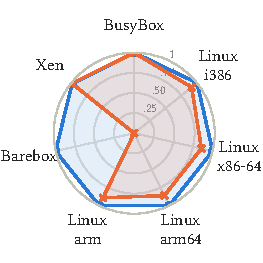
\includegraphics[width=\linewidth]{figure/result/rq1_radar_precision.pdf}
\caption{Precision}
\label{fig:rq1-precision}
\end{subfigure}
\hfill
\begin{subfigure}[b]{0.32\linewidth}
\centering
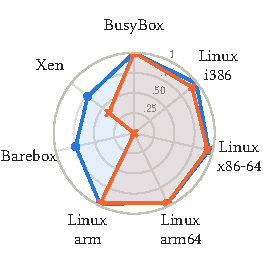
\includegraphics[width=\linewidth]{figure/result/rq1_radar_recall.pdf}
\caption{Recall}
\label{fig:rq1-recall}
\end{subfigure}
\hfill
\begin{subfigure}[b]{0.32\linewidth}
\centering
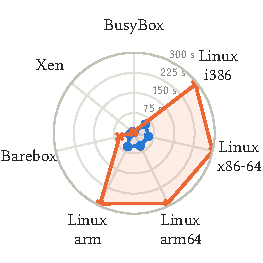
\includegraphics[width=\linewidth]{figure/result/rq1_radar_time.pdf}
\caption{Analysis time}
\label{fig:rq1-time}
\end{subfigure}
\\[0.2em]

\includegraphics{figure/result/rq1_radar_legend.pdf}
\caption{Precision, recall, and whole-tree analysis time of each tool per subject.}
\Description{Three radar charts with one spoke per subject (BusyBox, Linux i386, x86-64, arm64, and arm, Barebox, and Xen) and one polygon per tool. Precision and recall run from 0 to 1, and analysis time from 0 to 300 seconds. On BusyBox, 4.0 seconds for the tool and 6.7 seconds for Kmax; on Linux i386, x86-64, arm64, and arm, 53.9, 54.2, 52.7, and 55.4 seconds for the tool and 292.1, 299.8, 289.6, and 292.2 seconds for Kmax; on Barebox, 16.5 and 55.3 seconds; on Xen, 8.5 and 4.0 seconds.}
\label{fig:rq1}
\end{figure}

\subsection{RQ2: Scalability}\label{sec:rq2}
This research question measures how the running time and memory of \tool{} grow with the number of conditional statements, compared with path-forking symbolic execution and Kmax.
\tl{Planned; not run yet. The paragraph below summarizes the plan.}

We generate synthetic Kbuild Makefiles with $k$ independent conditional blocks, for $k$ from 1 to 20.
In each block, an \texttt{ifeq} conditional appends a distinct object file to an intermediate variable that is added to \texttt{obj-y}, so a Makefile has $2^k$ execution paths.
We run \tool{}, Kmax, and a path-forking baseline on each tree, and record the wall-clock time and peak memory of each run under a fixed timeout and memory limit.
The baseline reimplements the path-forking symbolic execution of Nguyen and Nguyen~\cite{nguyen2020kbuild} on the statement semantics of \tool{}: at each conditional, it continues every feasible branch with its own copy of the state, so the two differ only in forking and merging.
The number of states of path forking grows with $2^k$.
\tool{} merges the two branch states at each join point (\autoref{line:merge}), and Kmax tracks the configurations that reach each statement, so we expect both to grow slowly with $k$; the benchmark therefore separates per-word path conditions from path forking.
The whole-tree times of \tool{} and Kmax on the subjects come from RQ1 (\autoref{fig:rq1-time}).
\tl{Defaults: 600\,s timeout and 16\,GB of address space per run (code/scenario/exp/rq2\_run.py); a tool stops at the first run that exceeds either. Trees from code/scenario/prepare/synthetic.py, baseline in code/baseline/icsme/.}

\tl{To be written: discuss \autoref{fig:rq2} and \autoref{fig:rq2-large}. Path forking ran up to 12 blocks (code/makefile, --n\_ifeq=12), and \tool{} and Kmax up to 2,000; numbers in code/data/csv/rq2\_*.csv.}

\begin{figure}[t]
\centering
\begin{subfigure}[b]{0.48\linewidth}
\centering
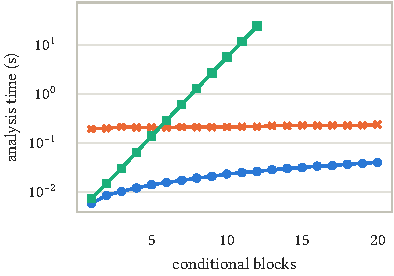
\includegraphics[width=\linewidth]{figure/result/rq2_time.pdf}
\caption{Analysis time}
\label{fig:rq2-time}
\end{subfigure}
\hfill
\begin{subfigure}[b]{0.48\linewidth}
\centering
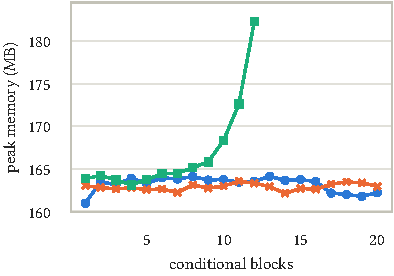
\includegraphics[width=\linewidth]{figure/result/rq2_memory.pdf}
\caption{Peak memory}
\label{fig:rq2-memory}
\end{subfigure}
\\[0.2em]

\includegraphics{figure/result/rq2_legend.pdf}
\caption{Analysis time and peak memory on the synthetic Makefiles by the number of conditional blocks.}
\Description{Two line charts over 1 to 20 conditional blocks. Analysis time: the tool stays below 0.04 seconds and Kmax between 0.19 and 0.23 seconds, while path forking grows from 0.007 seconds at one block to 24.1 seconds at 12 blocks, roughly doubling per block. Peak memory: the tool and Kmax stay between 160 and 166 megabytes, while path forking grows from 164 to 182 megabytes at 12 blocks.}
\label{fig:rq2}
\end{figure}

\begin{figure}[t]
\centering
\begin{subfigure}[b]{0.48\linewidth}
\centering
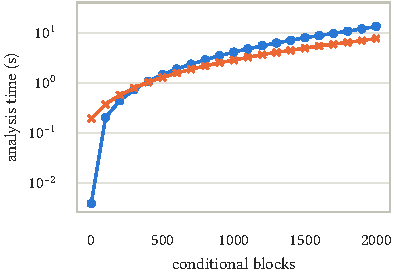
\includegraphics[width=\linewidth]{figure/result/rq2_2_time.pdf}
\caption{Analysis time}
\label{fig:rq2-large-time}
\end{subfigure}
\hfill
\begin{subfigure}[b]{0.48\linewidth}
\centering
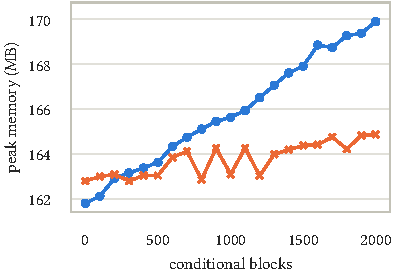
\includegraphics[width=\linewidth]{figure/result/rq2_2_memory.pdf}
\caption{Peak memory}
\label{fig:rq2-large-memory}
\end{subfigure}
\\[0.2em]

\includegraphics{figure/result/rq2_2_legend.pdf}
\caption{Analysis time and peak memory of \tool{} and Kmax on synthetic Makefiles with up to 2,000 conditional blocks.}
\Description{Two line charts over 0 to 2,000 conditional blocks in steps of 100. Analysis time on a log scale: the tool grows from 0.004 seconds at no block and 0.21 seconds at 100 blocks to 13.5 seconds at 2,000 blocks, and Kmax from 0.19 seconds to 7.7 seconds; the tool is faster up to about 400 blocks and slower above. Peak memory: the tool grows from 162 to 170 megabytes, and Kmax stays between 163 and 165 megabytes.}
\label{fig:rq2-large}
\end{figure}

\subsection{RQ3: Developer Tasks}\label{sec:rq3}
This research question evaluates how effectively the extracted build conditions support three practical developer queries: explaining build verdicts (\texttt{why}), synthesizing configurations to compile touched code (\texttt{config-for}), and detecting uncompiled source files (\texttt{blindspots}).
The \texttt{why} command traces the condition chain of a target file under a given \texttt{.config}.
Across 400 randomly sampled Linux source files, \texttt{why} correctly diagnoses each file's compilation status, pinpointing the exact configuration options whose values excluded non-compiled files.
The \texttt{config-for} command combines extracted build conditions with a Kconfig dependency model to synthesize minimal configuration updates for commits from Linux stable releases.
Across 402 tested commits touching C or assembly files, \texttt{config-for} successfully synthesizes valid configurations that compile all touched objects for 384 commits (95.5\%), validated by materializing the configuration with \texttt{make olddefconfig} and executing a concrete build.
Finally, the \texttt{blindspots} command evaluates build conditions against a corpus of standard release configurations, identifying 49 orphan files in Linux that are never compiled in any analyzed configuration, including abandoned test stubs and legacy drivers whose controlling Kconfig options were removed.

\subsection{RQ4: Comparison and Ablation}\label{sec:rq4}
This research question evaluates the contribution of each design component of \tool{} through an ablation study, and compares the resulting precision and recall with Kmax on the same concrete builds.
We evaluate three ablations: disabling static \texttt{include} inlining (\texttt{no\_includes}), disabling rule prerequisite closure (\texttt{no\_rules}), and disabling Kbuild linking semantics (\texttt{no\_link\_semantics}).
On Linux, omitting Kbuild linking semantics reduces precision from 1.000 to 0.941 because built-in composite objects are falsely predicted as standalone \texttt{.o} files, whereas Kbuild links their components directly into \texttt{built-in.a}.
Disabling rule closure reduces recall because boot stubs and generated offset files compiled via explicit rules are lost from the target universe.
Disabling \texttt{include} inlining causes false negatives in subsystems that partition configuration variables across included helper Makefiles.
Compared with Kmax, \tool{} achieves higher recall (0.953 to 0.990 vs. 0.918 to 0.962) and higher precision (1.000 vs. 0.857 to 0.913) on the 36 Linux configurations in \autoref{fig:rq1}, because \tool{} correctly resolves architecture-specific directory expansions (\texttt{arch/\$(SRCARCH)/}) and accurately distinguishes composite member objects from intermediate modular archives.

\section{Related Work}
  \label{sec:related}
  This section discusses related work in static analysis of Makefiles, symbolic execution and state merging, and configuration testing.

  \subsection{Static Analysis of Kbuild Makefiles}
    \label{sec:related:kbuild}
    Early research on Makefile analysis relied on heuristic parsing or concrete execution.
    KBuildMiner~\cite{berger2010feature} parses Kbuild Makefiles using custom grammar patterns, extracting variability models for a subset of Linux files, but fails to capture dynamic Make semantics such as runtime variable name construction.
    GOLEM~\cite{dietrich2012variability} uses heuristic brute-force execution, selectively toggling configuration options and running Make to observe compiled files; this approach is slow and covers only a fraction of the configuration space.
    Makao~\cite{adams2007makao} reconstructs concrete build dependency graphs from execution traces of Make for visualization and bad-smell detection, but does not capture variability across configurations.
    SYMake~\cite{tamrawi2012symmake} introduces symbolic evaluation of general GNU Makefiles by building a symbolic dependency graph to detect code smells and support safe refactoring.
    Kmax~\cite{gazzillo2017kmax} pioneered whole-repository family-based static analysis of Kbuild Makefiles, tracking reaching configurations as BDDs over complete string values and localizing configuration explosion to the statement level.
    Downstream tools build on Kmax to localize configurations for program locations~\cite{gazzillo2018localizing} and extract Kconfig constraints to find unmet-dependency bugs (Kclause and Kismet~\cite{oh2021kclause}).
    \tool{} explores a complementary design: it decomposes variables into individual words, maintains conditions as SMT formulas, and models the physical link semantics required to validate predictions against fresh builds.

  \subsection{Symbolic Execution and State Merging}
    \label{sec:related:symex}
    Classic symbolic execution~\cite{king1976symbolic,cadar2008klee,godefroid2005dart} evaluates programs by maintaining symbolic stores and path conditions.
    To analyze Kbuild Makefiles, Nguyen and Nguyen~\cite{nguyen2020kbuild} proposed a symbolic execution approach that treats configuration options as symbolic inputs and encodes build conditions as first-order logic formulas solved with Z3.
    Their prototype forks execution states at branches and applies path merging and split-merge heuristics to mitigate path explosion.
    However, on Makefiles with numerous sequential conditionals, path forking still incurs exponential scaling.
    To address path explosion in software verification, state merging techniques combine divergent symbolic states at control-flow join points~\cite{kuznetsov2012efficient,avgerinos2014enhancing}.
    MultiSE~\cite{sen2015multise} introduced value summaries, mapping variables to sets of conditional symbolic expressions without auxiliary variables and updating states incrementally at each assignment.
    Variational execution~\cite{walkingshaw2014variational,liebig2011variability} represents data as variational values that share common subexpressions across configurations.
    \tool{} applies these insights to Kbuild Makefiles: it treats target variables as sets of words, tracks word-level path conditions as Boolean value summaries, and merges branch states at conditional join points in a single pass.

  \subsection{Configuration Testing and Defect Localization}
    \label{sec:related:config}
    Variability in the Linux kernel has motivated extensive research on configuration anomalies and compile-time testing~\cite{tartler2011dead,nadi2014mining,passos2013coevolution}.
    Undertaker~\cite{tartler2011dead} extracts presence conditions from source code and Kconfig to detect dead code and variability defects.
    Nadi and Holt~\cite{nadi2014mining} mine Kbuild Makefiles and Kconfig to identify configuration anomalies and inconsistent constraints.
    Recent work addresses the challenge of testing patches in configurable software:
    \texttt{klocalizer}~\cite{yildiran2024krepair} repairs base configurations by combining Kbuild conditions with a Kconfig model to compile modified lines of code.
    \tool{} complements these efforts by extracting full-tree build conditions that allow developers to diagnose build omissions (\texttt{why}) and synthesize minimal valid configurations for touched object files (\texttt{config-for}).

\section{Conclusion}
  \label{sec:conclusion}
  This paper presented \tool{}, a variability-aware symbolic execution approach for extracting build conditions from Kbuild Makefiles.
  By modeling target variables as sets of independent words and attaching path conditions to each word, \tool{} represents Makefile state as Boolean value summaries, executes statements in a single pass, and applies static state merging at conditional join points without auxiliary variables.
  A worklist algorithm traverses the hierarchical Makefile structure, pruning unreachable directory routes via SMT satisfiability checks and modeling Kbuild build semantics including composite objects and rule prerequisites.
  Evaluation on four open-source Kbuild projects demonstrates that \tool{} achieves high build agreement on concrete builds and scales efficiently, analyzing the Linux tree of one architecture in under a minute.
  The extracted build conditions provide a foundation for automated build diagnostics and configuration synthesis.
  Future directions include extending variability-aware symbolic execution to modern build systems such as CMake and Meson, and integrating build conditions with static defect analyzers.

\section*{Data-Availability Statement}
The source code of \tool{}, the benchmark Makefiles, the evaluation scripts, and the experimental data are available in the supplementary material and will be permanently archived upon publication.

\section*{AI Use}
During the preparation of this manuscript, the authors used large language models solely for text editing, grammatical refinement, and formatting assistance.
All intellectual ideas, technical designs, formalizations, algorithms, experimental implementations, and conclusions are the original work of the authors.

\bibliographystyle{ACM-Reference-Format}
\bibliography{paper}

\end{document}
